\documentclass[12pt]{article}
\usepackage{graphicx,color}
\usepackage[margin=0.75in]{geometry}
\usepackage{amssymb}
\usepackage{footnote, enumerate, url, amsmath}
\usepackage{natbib}
\usepackage{multirow}
\usepackage{tabularx}
\usepackage{hyperref}
\usepackage{amssymb}

\hypersetup{
    colorlinks,
    citecolor=black,
    filecolor=black,
    linkcolor=black,
    urlcolor=black
}

\usepackage{titling}
\newcommand{\subtitle}[1]{%
  \posttitle{%
    \par\end{center}
    \begin{center}\large#1\end{center}
    \vskip0.5em}%
}

\def\starpy {\textsc{starpy}}


\begin{document}

\title{Summary of PhD Research}
\subtitle{\emph{The influence of morphology, AGN and environment on the quenching histories of galaxies}}
\author{Rebecca Smethurst}

\maketitle


What drives the evolution of galaxies from the disc dominated, star forming blue cloud to the elliptical dominated, quiescent red sequence? What role does the morphology, central supermassive black hole and galaxy environment play in this transition? 
% How do you answer them? STARPY?

In my thesis, I attempted to answer these questions by using Bayesian statistics to infer a simple star formation history (SFH) describing the time, $t_q$, and exponential rate, $\tau$, that star formation shuts down (often referred to as star formation quenching) in a galaxy. This statistical approach allowed me to reveal the subtle morphologically dependent evolutionary pathways taken by galaxies of all colours, shapes and environments. These conclusions are contradictory to previous studies suggesting that galaxy evolution is purely bimodal, with elliptical galaxies quenching rapidly and disc galaxies quenching slowly. Instead I was able to infer the broad range of quenching rates occuring across the diverse galaxy population. 

For a single galaxy, I used the optical photometry, provided by the Sloan Digital Sky Survey (SDSS), and the near ultra-violet (NUV) photometry, from the GALEX survey, in order to infer the posterior distribution of its SFH across the two dimensional $[t_q, \tau]$ parameter space. I then utilised the Galaxy Zoo 2 morphological classifications to obtain a morphology weighted, combined population distribution across each quenching parameter for a sample of galaxies. 
% What do you find in morph chapter?

I applied this method across the blue cloud, green valley and red sequence of a sample of $126,316$ galaxies and found a clear difference between the quenching timescales preferred by smooth and disc weighted populations, with three major routes through the green valley dominated by smooth (rapid rates, attributed to major mergers), intermediately classified (intermediate rates, attributed to galaxy interactions) and disc morphologies (slow rates, attributed to secular, i.e. slow, processes). I hypothesised that morphological changes occur in systems which have undergone quenching with an exponential rate, $\tau < 1.5~\rm{Gyr}$, in order for the evolution of galaxies in the green valley to match the ratio of smooth to disc galaxies observed in the red sequence.
% What do you find in AGN feedback chap?

Along with the morphological dependence of galaxy evolution, the active central supermassive black hole of a galaxy (an active galactic nucleus; AGN) is thought to affect a galaxy's star formation rate in a process known as AGN feedback. AGN feedback was first suggested as a mechanism for regulating star formation due to the results of simulations wherein galaxies could grow to unrealistic stellar masses. This stellar mass build up is thought to occur through many mergers of galaxies over cosmic time, a process which AGN feedback can regulate by either rapidly expelling or heating the gas needed for further star formation, causing a quench and reducing the ultimate stellar mass of a galaxy. So far, only indirect observational evidence has been found for AGN feedback, the strongest being the indirect evidence that the largest AGN fraction is found in the green valley (Cowie \& Barger, 2008; Hickox et al., 2009; Schawinski et al., 2010), suggesting a link between AGN activity and the process which moves a galaxy from the blue cloud to the red sequence.

I therefore repeated my SFH analysis for a sample of $1,244$ obscured AGN host galaxies and found statistical evidence for recent, rapid quenching, suggesting that this may be caused by AGN feedback. This result is shown by the population distributions shown in Figure~\ref{fig:agnfeedback}. This result is the first statistically supported observational evidence for AGN feedback in a population of galaxies. 

\begin{figure*}
\centering{
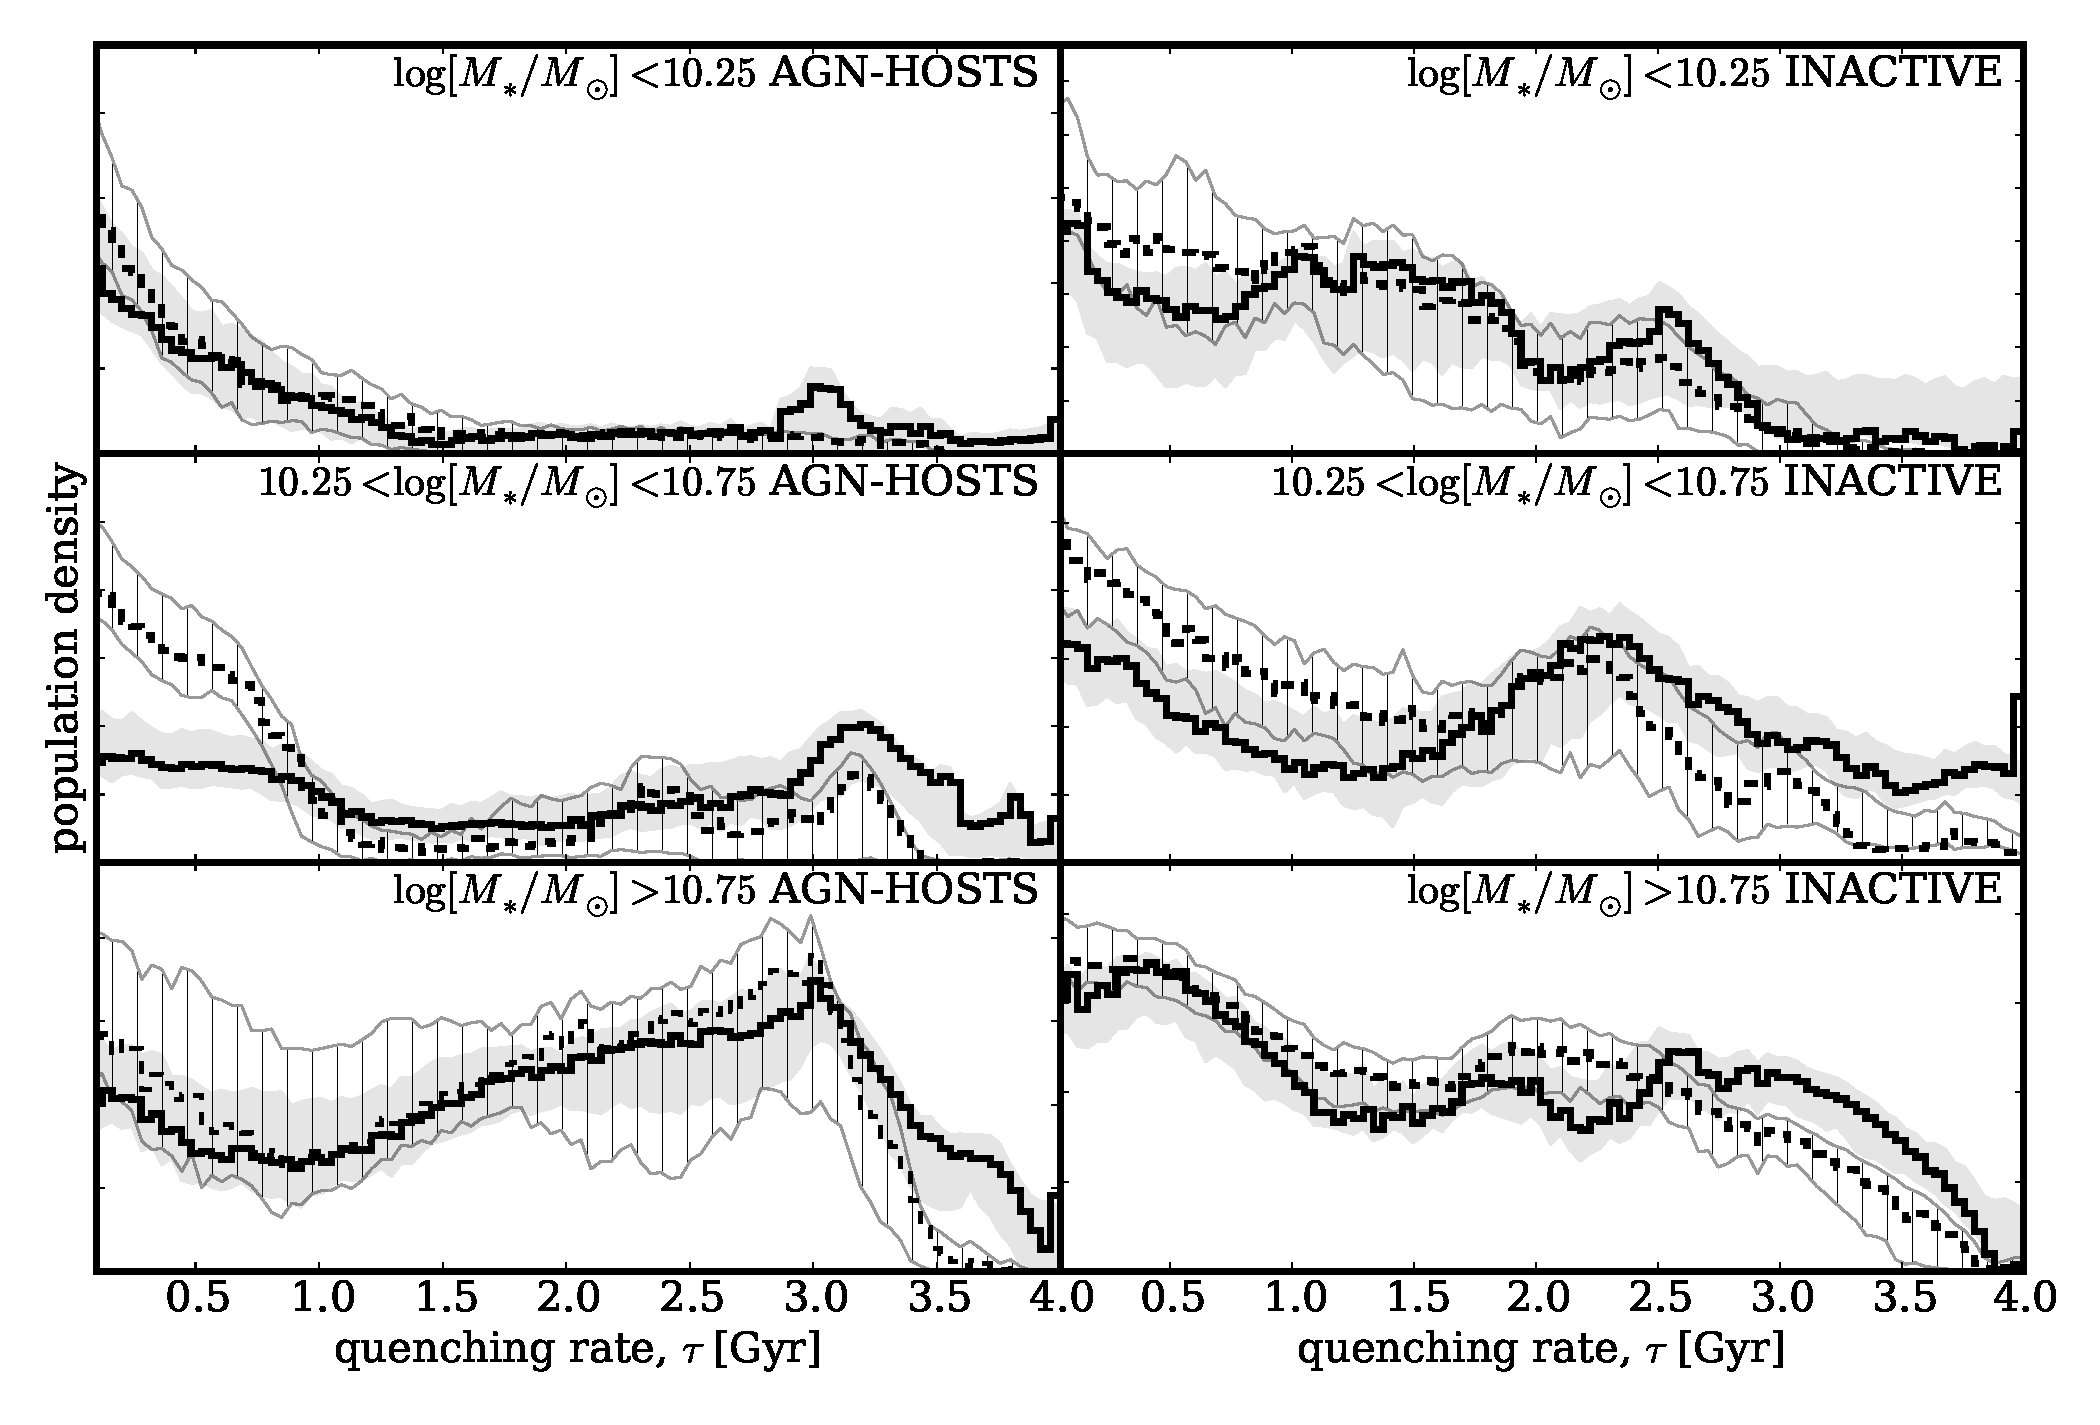
\includegraphics[width=\textwidth]{fig5.pdf}}
\caption[Quenching rate population density distributions for the \textsc{agn-host} and \textsc{inactive} samples]{Population density distributions for the quenching rate ($\tau$). The curves are normalised so that the areas under the curves in a single panel are equal. \textsc{agn-host} (left) host and \textsc{inactive} (right) galaxies are split into low (top), medium (middle) and high (bottom) mass for smooth (dashed) and disc (solid) galaxies. Uncertainties from bootstrapping are shown by the shaded regions for the smooth (grey striped) and disc (grey solid) population densities. A small (large) value of $\tau$ corresponds to a rapid (slow) quench.}
\label{fig:agnfeedback}
\end{figure*}

However, I also found that rapid quenching rates cannot account for all the quenching across the AGN host population; slow quenching rates, attributed to secular evolution, are also significant in the evolution of AGN host galaxies. This is contrary to many previous works suggesting that the bulk of galaxy-black hole co-evolution occurs in violent processes such as mergers which simultaneously grow the black hole and galaxy, in particular the central stellar bulge component of a galaxy. Conversely, slow secular processes would not be able to significantly grow the black hole significantly in order for it to have enough energy to cause feedback on the galaxy.
% What do you find in bulgeless AGN?

I investigated this possible secular co-evolution of galaxies and black holes further by measuring the black hole masses of a sample of $101$ bulgeless AGN host galaxies. Bulgeless galaxies are thought to arise due to a lack of bulge building mergers in a galaxy's evolutionary history. I compared the black hole masses of these bulgeless galaxies to those of typical galaxies and compared their locations on well known black hole-galaxy scaling relations, as shown in Figure~\ref{fig:bulgevsbh}. I found that the measured black holes of the bulgeless galaxies are $\sim1-2~\rm{dex}$ more massive than they should be, given their lack of bulges. However, I also found that the measured black holes of these bulgeless galaxies are appropriate for the total stellar mass of their host galaxies. This suggests that black hole-galaxy scaling relations may arise due to mutual correlations to the overall gravitational potential of the dark matter halo of the galaxy, contradicting the long held theory that black holes only grow to large masses during galaxy mergers. 

\begin{figure*}
\centering
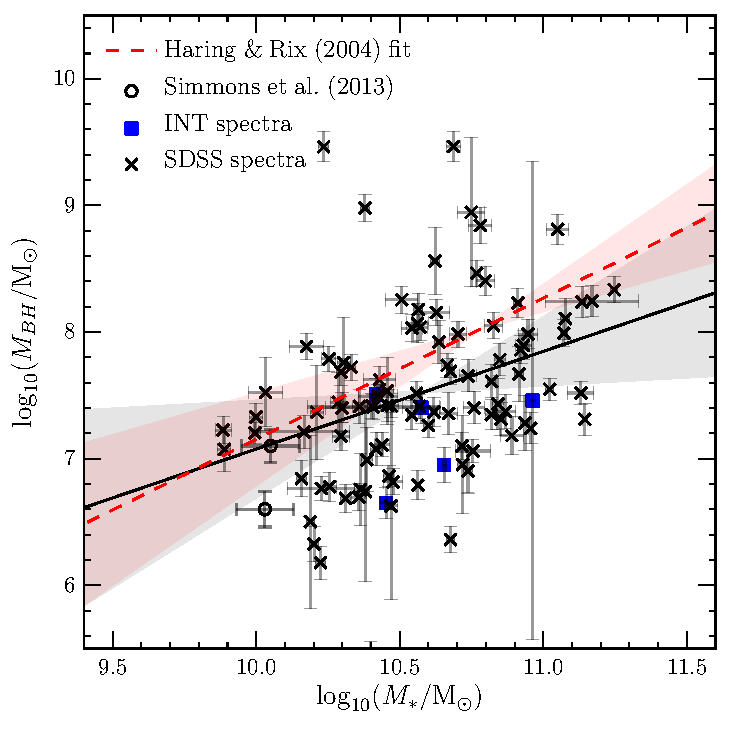
\includegraphics[width=0.48\textwidth]{mass_bh_total_mass_fit_linmix_fit.pdf}
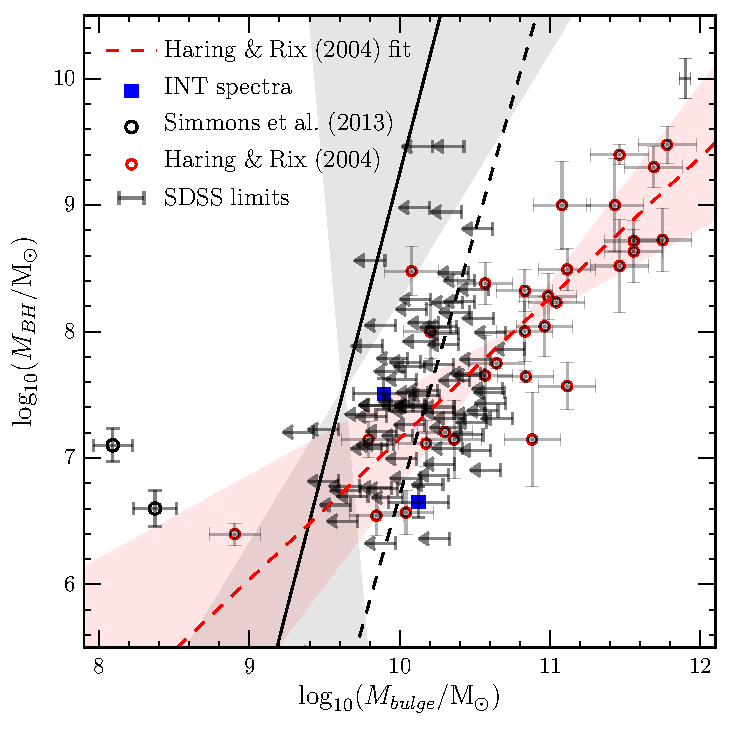
\includegraphics[width=0.48\textwidth]{mass_bh_bulge_limits_INT_simmons13_measurements_linmix_fit.pdf}
\caption{Total stellar mass (left) and upper limits on the bulge against the black hole mass of the 101 \textsc{bulgeless} galaxies (crosses and blue squares) and detections from Simmons et al. (2013; open circles). The best fit line to the data points and two-dimensional errors from linear regression is shown (solid line) with $\pm3\sigma$ (grey shaded). I also show the best fit found using this same method to the early-type galaxies of Haring \& Rix (2004; dashed line) with $\pm3\sigma$ (red shaded) and the measured values shown by the red circles. The upper limits on the calculated stellar bulge masses are plotted (right) against the black hole mass for the \textsc{bulgeless} sample. The best fit to these upper limits and two-dimensional errors using linear regression methods (solid line) is shown with $\pm3\sigma$ (grey shaded). The dashed line shows the fit if the upper limits are not treated as such. I also show the best fit found using this same method to the early-type galaxies of Haring \& Rix (2004; dashed line) with $\pm3\sigma$ (red shaded) and the measured values shown by the red circles.
}
\label{fig:bulgevsbh}
\end{figure*}
% What do you find in environment chapter?

I also considered the effect of the group environment on the time and rate that quenching occurs, with respect to the group-centric radius, for $4,629$ satellite galaxies. I found that although mergers, mass quenching and morphological quenching are all occurring in groups, environmentally driven quenching mechanisms are also prevalent. However, I find that these environmentally driven quenching processes are not correlated with the velocity of a satellite within a group, ruling out ram pressure stripping as a possible quenching mechanism. 
% Sum up your big picture

I discussed in detail how all of these quenching mechanisms are likely to affect a galaxy across its lifetime, acting in concert to reduce the SFR, which in turn produces the wide distribution of quenching timescales seen across the colour-magnitude diagram. I discussed ideas for future work using the method employed in this work, including applying it to forthcoming data from large integral field unit surveys, which I am currently working towards during my research fellowship. 

\end{document}t